\documentclass[10 pt,usenames,dvipsnames, oneside]{article}
\usepackage{../../../modelo-ensino-medio}



\begin{document}

\begin{center}
  \begin{minipage}[l]{3cm}

\includegraphics[width=2cm]{logo}    
\end{minipage}\hfill
\begin{minipage}[r]{.8\textwidth}
 {\Large \scshape Atividade: Rio Star}  
\end{minipage}
\end{center}
\vspace{.2cm}

% \ifdefined\prof
% %Habilidades da BNCC
% % \begin{objetivos}
% % \item 
% % \end{objetivos}

% %Caixa do Para o Professor
% \begin{goals}
% %Objetivos específicos
% \begin{enumerate}
% \item
% \end{enumerate}

% \tcblower

% %Orientações e sugestões
% \begin{itemize}
% \item 
% \end{itemize}
% \end{goals}

% \bigskip
% \begin{center}
% {\large \scshape Atividade}
% \end{center}
% \fi

\begin{figure}[H]
\centering

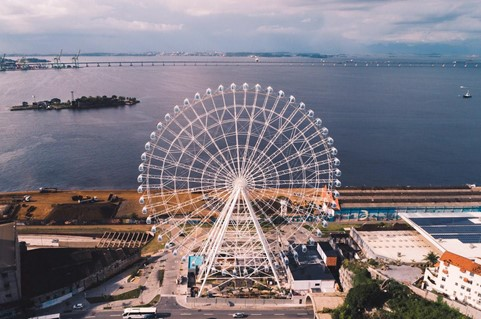
\includegraphics[width=.75\linewidth]{trigonometricas18}
\end{figure}

A Rio Star é a maior roda gigante da América Latina e está localizada na cidade do Rio de Janeiro. Ela tem $88$ metros de altura. A atração turística conta com $54$ cabines climatizadas que podem receber até 8 pessoas cada, totalizando $432$ visitantes que poderão apreciar a vista da Zona Portuária, do Relógio Central, Morro da Providência, Cristo Redentor, Pão de Açúcar, Pedra do Sal, Ponte Rio-Niterói e da Cidade do Samba durante 18 minutos - tempo necessário para a volta completa no brinquedo. (Fonte: \href{https://casavogue.globo.com/LazerCultura/Viagem/noticia/2019/12/rio-star-roda-gigante-do-rio-de-janeiro-inaugura-hoje.html}{Casa Vogue})

Suponha que o ponto mais baixo da roda gigante que qualquer uma das cabines pode atingir se encontra a $3$ metros de altura do chão. Beatriz e Gabriela embarcam em uma das cabines e a partir daí, a roda gigante gira continuamente com a mesma velocidade e dá duas voltas sem parar, finalizando o movimento com a cabine das meninas retornando ao ponto mais baixo.

\begin{enumerate}
\item Qual é o raio da roda gigante?
\item Existe algum momento em que a altura da cabine em relação ao chão será nula? Justifique.
\item Em quais instantes do movimento a cabine estará na mesma altura do centro da roda gigante? E no ponto mais alto da roda? E no ponto mais baixo?
\item Você acha que a altura a que a cabine sobe nos primeiros dois minutos do movimento é a mesma que nos dois minutos seguintes? Justifique sua resposta?
\item No plano cartesiano, plote no plano cartesiano os pontos $(t,h)$ com os dados obtidos no item \titem{c)}, em que $t$ é o tempo e $h$ é a altura da cabine. Em seguida, esboce a curva por meio desses pontos que você acha que representa o gráfico da função altura $h = h(t)$. Compare seu gráfico com o de seus colegas.
\item Qual o período, a amplitude e o conjunto imagem da função $h = h(t)$?
\end{enumerate}


\ifdefined\prof
\begin{solucao}

\begin{enumerate}
	\item $42{,}5$ mts
	\item Não, pois o ponto mais baixo da roda gigante está a $3$ mts
	do chão
	\item Mesma altura do centro: $4$ min e $30$ seg, $13$ min e $30$ seg,
	$22$ min e $30$ seg e $31$ min e $30$ seg.

	Pontos mais altos: $9$ e $27$ min

	Pontos mais baixos: $0$, $18$ e $36$ min
	\item Não. No intervalo $[0; 4{,}5]$ do tempo, a cadeira parte da
	posição mais baixa na roda gigante e gira um quarto de volta,
	atingindo a altura do centro da roda. Nos dois minutos
	iniciais, a cadeira se encontra no ponto mais baixo da roda e
	quando esta começa a girar, o deslocamento horizontal da
	cabine inicialmente será maior que o vertical. Nos dois
	minutos seguintes, a situação se inverte, aumentando mais o
	deslocamento vertical da cadeira em relação ao horizontal.
	Portanto, nos primeiros dois minutos de movimento a cadeira
	subirá uma altura menor que nos dois minutos seguintes.
	\item Período: $18$; Imagem: $[3;88]$; amplitude: $42{,}5$
	\end{enumerate}

\end{solucao}
\fi

\end{document}